This appendix contains all the graphs and the tables related to the read experiments conducted, and of the comparison with the related work. Results are reported first expressed as latency (measured in seconds) and then as throughput (measured in rows/seconds). Latency was directly measured, while throughput was computed from the latency and table size.

%%%%%%%%%%%%%%%%%%%%%%%%%%%%%%%%%%%%%%%%%%%%%%%%%%%%%%%%%%%%%%%%%
%%%%%%%%%%%%              LATENCY             %%%%%%%%%%%%%%%%%%%
%%%%%%%%%%%%%%%%%%%%%%%%%%%%%%%%%%%%%%%%%%%%%%%%%%%%%%%%%%%%%%%%%
\begin{figure}
    \centering
    \begin{minipage}[b]{\textwidth}
        \centering
        \captionof{table}[Read experiment - Latency - 1 CPU core]{Read experiment results expressed as latency. The experiment was performed with one \glstext{CPU} core.}
        \label{tbl:appx_res_read_time_1_core_HID}
        \begin{tabular}{c r S[table-format=5.5] S[table-format=5.5] S[table-format=5.5]} 
            \toprule
            \multirow{2}{*}{{Pipeline\Tstrut\Bstrut}} & \multirow{2}{*}{{\thead{Number\\ of rows}}} & {\multirow{2}{*}{{\thead{Latency \\ (seconds)}}}} & \multicolumn{2}{c}{{\thead{Latency (seconds) \\95\% Confidence Interval}}}\\
                                                      &                                             &                                                   & {low} & {high}\\
            \midrule
            \multirow{5}{4em}{Hudi\\Legacy}         &   10K   &       0.63144  &       0.62360  &       0.64086  \\
                                                    &  100K   &       2.65043  &       2.64277  &       2.65880  \\
                                                    &    1M   &       8.59296  &       8.32432  &       8.88965  \\
                                                    &    6M   &      33.52580  &      33.22121  &      33.83881  \\
                                                    &   60M   &      33.69031  &      33.34263  &      34.03532  \\
            \midrule
            \multirow{5}{4em}{Iceberg\\PyIceberg}   &   10K   &       0.01723  &       0.01646  &       0.01799  \\
                                                    &  100K   &       0.04687  &       0.04283  &       0.05107  \\
                                                    &    1M   &       0.43018  &       0.41987  &       0.44190  \\
                                                    &    6M   &       2.12331  &       2.10768  &       2.13933  \\
                                                    &   60M   &      21.81955  &      21.69884  &      21.93705  \\
            \midrule
            \multirow{5}{4em}{Delta Lake\\delta-rs} &   10K   &       0.05345  &       0.03917  &       0.08056  \\
                                                    &  100K   &       0.05763  &       0.05505  &       0.06055  \\
                                                    &    1M   &       0.53878  &       0.52444  &       0.55318  \\
                                                    &    6M   &       1.94947  &       1.92855  &       1.96958  \\
                                                    &   60M   &      22.98186  &      22.83994  &      23.15794  \\
            \bottomrule
        \end{tabular}
    \end{minipage}
    \begin{minipage}[b]{\textwidth}
        \centering
        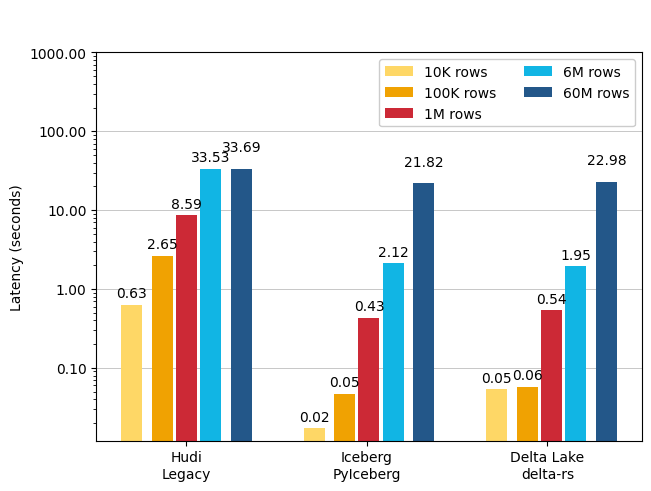
\includegraphics[width=\textwidth]{figures/7-appendix/results_diagrams/read/hudi_iceberg_delta/read_time_1_core.png}
        \caption[Histogram of the read experiment - Latency - 1 CPU core]{Histogram in log-scale of the read experiment results expressed as latency. The experiment was performed with one \glstext{CPU} core.}
        \label{fig:appx_res_read_time_1_core_HID}
    \end{minipage}
\end{figure}


\begin{figure}
    \centering
    \begin{minipage}[b]{\textwidth}
        \centering
        \captionof{table}[Read experiment - Latency - 2 CPU cores]{Read experiment results expressed as latency. The experiment was performed with two \glstext{CPU} cores.}
        \label{tbl:appx_res_read_time_2_cores_HID}
        \begin{tabular}{c r S[table-format=5.5] S[table-format=5.5] S[table-format=5.5]} 
            \toprule
            \multirow{2}{*}{{Pipeline\Tstrut\Bstrut}} & \multirow{2}{*}{{\thead{Number\\ of rows}}} & {\multirow{2}{*}{{\thead{Latency \\ (seconds)}}}} & \multicolumn{2}{c}{{\thead{Latency (seconds) \\95\% Confidence Interval}}}\\
                                                      &                                             &                                                   & {low} & {high}\\
            \midrule
            \multirow{5}{4em}{Hudi\\Legacy}         &   10K   &       0.62482  &       0.62181  &       0.62802  \\
                                                    &  100K   &       2.66332  &       2.65615  &       2.67070  \\
                                                    &    1M   &       8.60687  &       8.30138  &       8.97921  \\
                                                    &    6M   &      33.37740  &      33.09684  &      33.70681  \\
                                                    &   60M   &      33.62880  &      33.28617  &      34.01780  \\
            \midrule
            \multirow{5}{4em}{Iceberg\\PyIceberg}   &   10K   &       0.01832  &       0.01735  &       0.01931  \\
                                                    &  100K   &       0.04317  &       0.04143  &       0.04518  \\
                                                    &    1M   &       0.26943  &       0.26217  &       0.27664  \\
                                                    &    6M   &       1.29606  &       1.23003  &       1.34385  \\
                                                    &   60M   &      13.51294  &      13.41047  &      13.62477  \\
            \midrule
            \multirow{5}{4em}{Delta Lake\\delta-rs} &   10K   &       0.04121  &       0.03931  &       0.04385  \\
                                                    &  100K   &       0.05721  &       0.05110  &       0.06694  \\
                                                    &    1M   &       0.23373  &       0.22513  &       0.24263  \\
                                                    &    6M   &       0.90826  &       0.89900  &       0.91835  \\
                                                    &   60M   &      11.40975  &      11.27301  &      11.59608  \\
            \bottomrule
        \end{tabular}
    \end{minipage}
    \begin{minipage}[b]{\textwidth}
        \centering
        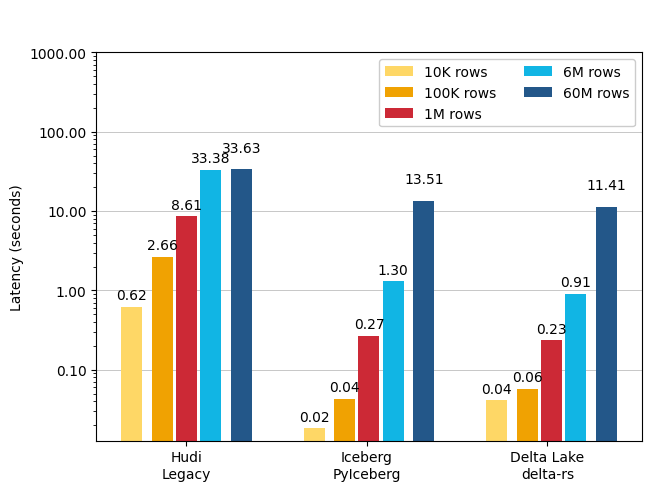
\includegraphics[width=\textwidth]{figures/7-appendix/results_diagrams/read/hudi_iceberg_delta/read_time_2_core.png}
        \caption[Histogram of the read experiment - Latency - 2 CPU cores]{Histogram in log-scale of the read experiment results expressed as latency. The experiment was performed with two \glstext{CPU} cores.}
        \label{fig:appx_res_read_time_2_cores_HI}
    \end{minipage}
\end{figure}

\begin{figure}
    \centering
    \begin{minipage}[b]{\textwidth}
        \centering
        \captionof{table}[Read experiment - Latency - 4 CPU cores]{Read experiment results expressed as latency. The experiment was performed with four \glstext{CPU} cores.}
        \label{tbl:appx_res_read_time_4_cores_HDI}
        \begin{tabular}{c r S[table-format=5.5] S[table-format=5.5] S[table-format=5.5]} 
            \toprule
            \multirow{2}{*}{{Pipeline\Tstrut\Bstrut}} & \multirow{2}{*}{{\thead{Number\\ of rows}}} & {\multirow{2}{*}{{\thead{Latency \\ (seconds)}}}} & \multicolumn{2}{c}{{\thead{Latency (seconds) \\95\% Confidence Interval}}}\\
                                                      &                                             &                                                   & {low} & {high}\\
            \midrule
            \multirow{5}{4em}{Hudi\\Legacy}         &   10K   &       0.63624  &       0.62355  &       0.65945  \\
                                                    &  100K   &       2.63986  &       2.63350  &       2.64647  \\
                                                    &    1M   &       8.74436  &       8.52235  &       9.00047  \\
                                                    &    6M   &      33.44749  &      33.18573  &      33.74060  \\
                                                    &   60M   &      33.66153  &      33.26312  &      34.09078  \\
            \midrule
            \multirow{5}{4em}{Iceberg\\PyIceberg}   &   10K   &       0.02979  &       0.01568  &       0.05914  \\
                                                    &  100K   &       0.04283  &       0.04113  &       0.04474  \\
                                                    &    1M   &       0.23337  &       0.21855  &       0.24806  \\
                                                    &    6M   &       1.00857  &       1.00123  &       1.01616  \\
                                                    &   60M   &      10.11029  &      10.04090  &      10.18332  \\
            \midrule
            \multirow{5}{4em}{Delta Lake\\delta-rs} &   10K   &       0.04357  &       0.03931  &       0.05102  \\
                                                    &  100K   &       0.05546  &       0.05372  &       0.05786  \\
                                                    &    1M   &       0.18958  &       0.15076  &       0.25524  \\
                                                    &    6M   &       0.53106  &       0.50752  &       0.56920  \\
                                                    &   60M   &       5.57990  &       5.54508  &       5.61830  \\
\bottomrule
        \end{tabular}
    \end{minipage}
    \begin{minipage}[b]{\textwidth}
        \centering
        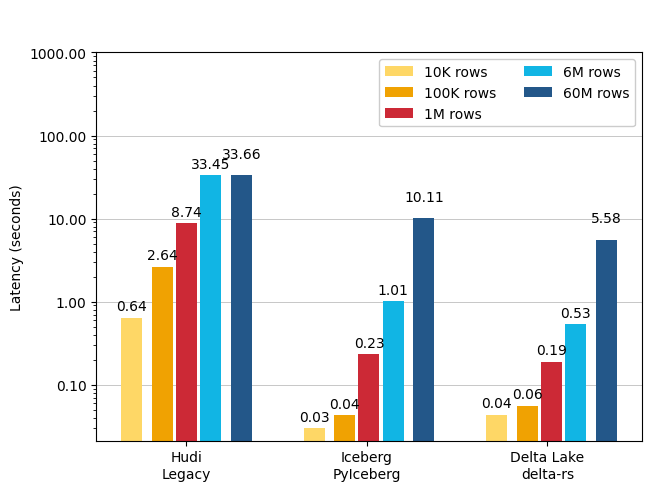
\includegraphics[width=\textwidth]{figures/7-appendix/results_diagrams/read/hudi_iceberg_delta/read_time_4_core.png}
        \caption[Histogram of the read experiment - Latency - 4 CPU cores]{Histogram in log-scale of the read experiment results expressed as latency. The experiment was performed with four \glstext{CPU} cores.}
        \label{fig:appx_res_read_time_4_cores_HID}
    \end{minipage}
\end{figure}

\begin{figure}
    \centering
    \begin{minipage}[b]{\textwidth}
        \centering
        \captionof{table}[Read experiment - Latency - 8 CPU cores]{Read experiment results expressed as latency. The experiment was performed with eight \glstext{CPU} cores.}
        \label{tbl:appx_res_read_time_8_cores_HID}
        \begin{tabular}{c r S[table-format=5.5] S[table-format=5.5] S[table-format=5.5]} 
            \toprule
            \multirow{2}{*}{{Pipeline\Tstrut\Bstrut}} & \multirow{2}{*}{{\thead{Number\\ of rows}}} & {\multirow{2}{*}{{\thead{Latency \\ (seconds)}}}} & \multicolumn{2}{c}{{\thead{Latency (seconds) \\95\% Confidence Interval}}}\\
                                                      &                                             &                                                   & {low} & {high}\\
            \midrule
            \multirow{5}{4em}{Hudi\\Legacy}         &   10K   &       0.62733  &       0.62254  &       0.63250  \\
                                                    &  100K   &       2.66235  &       2.65322  &       2.67216  \\
                                                    &    1M   &       8.35214  &       8.14163  &       8.61832  \\
                                                    &    6M   &      33.44013  &      33.16978  &      33.75254  \\
                                                    &   60M   &      33.14244  &      32.90073  &      33.40544  \\
            \midrule
            \multirow{5}{4em}{Iceberg\\PyIceberg}   &   10K   &       0.01696  &       0.01598  &       0.01810  \\
                                                    &  100K   &       0.04268  &       0.04096  &       0.04478  \\
                                                    &    1M   &       0.23212  &       0.22927  &       0.23531  \\
                                                    &    6M   &       0.88465  &       0.87563  &       0.89454  \\
                                                    &   60M   &       8.83920  &       8.75894  &       8.93390  \\
            \midrule
            \multirow{5}{4em}{Delta Lake\\delta-rs} &   10K   &       0.04314  &       0.03883  &       0.05129  \\
                                                    &  100K   &       0.05465  &       0.05299  &       0.05665  \\
                                                    &    1M   &       0.17409  &       0.16983  &       0.17829  \\
                                                    &    6M   &       0.49707  &       0.48562  &       0.51095  \\
                                                    &   60M   &       2.94431  &       2.85972  &       3.05301  \\
            \bottomrule
        \end{tabular}
    \end{minipage}
    \begin{minipage}[b]{\textwidth}
        \centering
        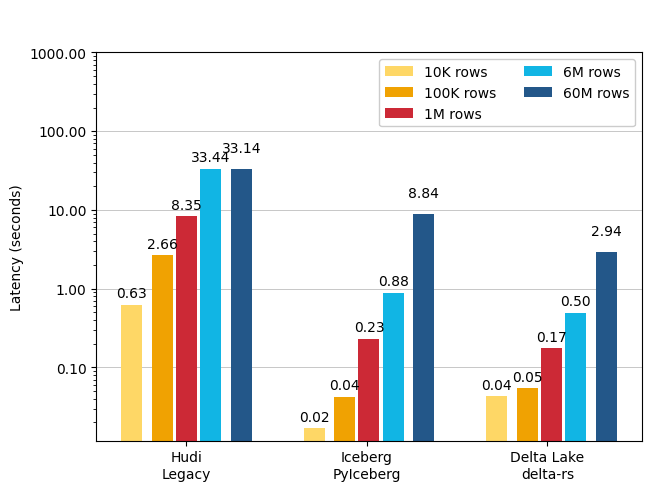
\includegraphics[width=\textwidth]{figures/7-appendix/results_diagrams/read/hudi_iceberg_delta/read_time_8_core.png}
        \caption[Histogram of the read experiment - Latency - 8 CPU cores]{Histogram in log-scale of the read experiment results expressed as latency. The experiment was performed with eight \glstext{CPU} cores.}
        \label{fig:appx_res_read_time_8_cores_HID}
    \end{minipage}
\end{figure}



%%%%%%%%%%%%%%%%%%%%%%%%%%%%%%%%%%%%%%%%%%%%%%%%%%%%%%%%%%%%%%%%%
%%%%%%%%%%%%             THROUGHPUT           %%%%%%%%%%%%%%%%%%%
%%%%%%%%%%%%%%%%%%%%%%%%%%%%%%%%%%%%%%%%%%%%%%%%%%%%%%%%%%%%%%%%%

\begin{figure}
    \centering
    \begin{minipage}[b]{\textwidth}
        \centering
        \captionof{table}[Read experiment - Throughput - 1 CPU core]{Read experiment results expressed as throughput. The experiment was performed with one \glstext{CPU} core.}
        \label{tbl:appx_res_read_throughput_1_core_HID}
        \begin{tabular}{c r S[table-format=5.5] S[table-format=5.5] S[table-format=5.5]} 
            \toprule
            \multirow{2}{*}{{Pipeline\Tstrut\Bstrut}} & \multirow{2}{*}{{\thead{Number\\ of rows}}} & {\multirow{2}{*}{{\thead{Throughput \\ (k rows/second)}}}} & \multicolumn{2}{c}{{\thead{Throughput (k rows/second) \\95\% Confidence Interval}}}\\
                                                      &                                             &                                                          & {low} & {high}\\
            \midrule
            \multirow{5}{4em}{Hudi\\Legacy}         &  10K  &     15.83673  &     15.60392  &     16.03591  \\
                                                    & 100K  &     37.72979  &     37.61100  &     37.83907  \\
                                                    &   1M  &    116.37431  &    112.49038  &    120.12997  \\
                                                    &   6M  &    178.96662  &    177.31121  &    180.60749  \\
                                                    &  60M  &   1780.92764  &   1762.87434  &   1799.49802  \\
            \midrule
            \multirow{5}{4em}{Iceberg\\PyIceberg}   &  10K  &    580.48003  &    555.59531  &    607.64551  \\
                                                    & 100K  &   2133.40362  &   1958.11912  &   2334.61316  \\
                                                    &   1M  &   2324.62963  &   2262.96750  &   2381.66201  \\
                                                    &   6M  &   2825.77691  &   2804.61249  &   2846.73095  \\
                                                    &  60M  &   2749.82753  &   2735.09913  &   2765.12511  \\
            \midrule
            \multirow{5}{4em}{Delta Lake\\delta-rs} &  10K  &    187.08171  &    124.12941  &    255.27425  \\
                                                    & 100K  &   1735.08031  &   1651.50261  &   1816.68579  \\
                                                    &   1M  &   1856.03325  &   1807.74307  &   1906.81184  \\
                                                    &   6M  &   3077.75801  &   3046.33018  &   3111.14548  \\
                                                    &  60M  &   2610.75520  &   2590.90390  &   2626.97689  \\
            \bottomrule
        \end{tabular}
    \end{minipage}
    \begin{minipage}[b]{\textwidth}
        \centering
        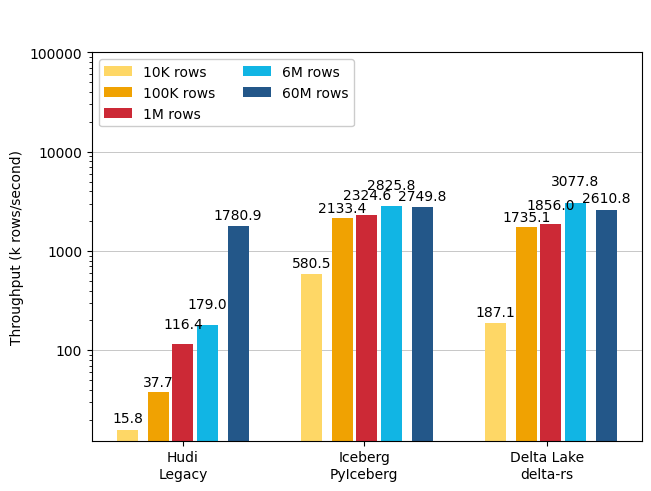
\includegraphics[width=\textwidth]{figures/7-appendix/results_diagrams/read/hudi_iceberg_delta/read_throughput_1_core.png}
        \caption[Histogram of the read experiment - Throughput - 1 CPU core]{Histogram in log-scale of the read experiment results expressed as throughput. The experiment was performed with one \glstext{CPU} core.}
        \label{fig:appx_res_read_throughput_1_core_HID}
    \end{minipage}
\end{figure}

\begin{figure}
    \centering
    \begin{minipage}[b]{\textwidth}
        \centering
        \captionof{table}[Read experiment - Throughput - 2 CPU cores]{Read experiment results expressed as throughput. The experiment was performed with two \glstext{CPU} cores.}
        \label{tbl:appx_res_read_throughput_2_cores_HID}
        \begin{tabular}{c r S[table-format=5.5] S[table-format=5.5] S[table-format=5.5]}  
            \toprule
            \multirow{2}{*}{{Pipeline\Tstrut\Bstrut}} & \multirow{2}{*}{{\thead{Number\\ of rows}}} & {\multirow{2}{*}{{\thead{Throughput \\ (k rows/second)}}}} & \multicolumn{2}{c}{{\thead{Throughput (k rows/second) \\95\% Confidence Interval}}}\\
                                                      &                                             &                                                          & {low} & {high}\\
            \midrule
            \multirow{5}{4em}{Hudi\\Legacy}         &  10K  &     16.00450  &     15.92295  &     16.08220  \\
                                                    & 100K  &     37.54712  &     37.44331  &     37.64842  \\
                                                    &   1M  &    116.18627  &    111.36842  &    120.46187  \\
                                                    &   6M  &    179.76235  &    178.00556  &    181.28617  \\
                                                    &  60M  &   1784.18508  &   1763.78251  &   1802.55061  \\
            \midrule
            \multirow{5}{4em}{Iceberg\\PyIceberg}   &  10K  &    545.75837  &    517.75702  &    576.36742  \\
                                                    & 100K  &   2316.16325  &   2213.60744  &   2413.48199  \\
                                                    &   1M  &   3711.54185  &   3614.79402  &   3814.37302  \\
                                                    &   6M  &   4629.43293  &   4464.78544  &   4877.93641  \\
                                                    &  60M  &   4440.18728  &   4403.74316  &   4474.11701  \\
            \midrule
            \multirow{5}{4em}{Delta Lake\\delta-rs} &  10K  &    242.64097  &    228.05610  &    254.40100  \\
                                                    & 100K  &   1747.92159  &   1493.97160  &   1957.12561  \\
                                                    &   1M  &   4278.42215  &   4121.53210  &   4441.78008  \\
                                                    &   6M  &   6606.02333  &   6533.47380  &   6674.05228  \\
                                                    &  60M  &   5258.66143  &   5174.16360  &   5322.44783  \\
            
            \bottomrule
        \end{tabular}
    \end{minipage}
    \begin{minipage}[b]{\textwidth}
        \centering
        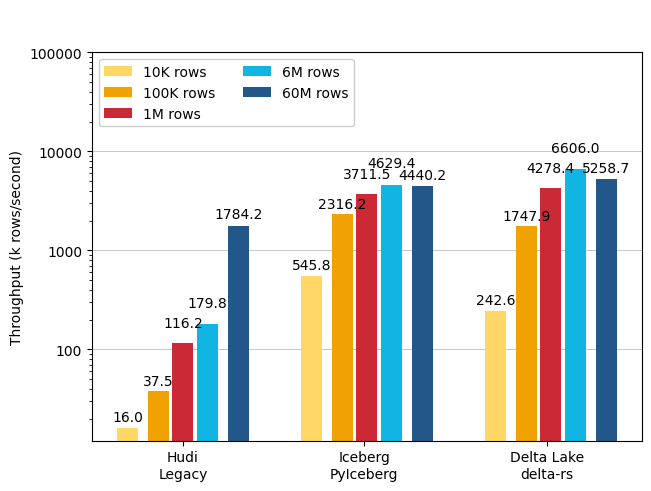
\includegraphics[width=\textwidth]{figures/7-appendix/results_diagrams/read/hudi_iceberg_delta/read_throughput_2_core.png}
        \caption[Histogram of the read experiment - Throughput - 2 CPU cores]{Histogram in log-scale of the read experiment results expressed as throughput. The experiment was performed with two \glstext{CPU} cores.}
        \label{fig:appx_res_read_throughput_2_cores_HID}
    \end{minipage}
\end{figure}

\begin{figure}
    \centering
    \begin{minipage}[b]{\textwidth}
        \centering
        \captionof{table}[Read experiment - Throughput - 4 CPU cores]{Read experiment results expressed as throughput. The experiment was performed with four \glstext{CPU} cores.}
        \label{tbl:appx_res_read_throughput_4_cores_HID}
        \begin{tabular}{c r S[table-format=5.5] S[table-format=5.5] S[table-format=5.5]} 
            \toprule
            \multirow{2}{*}{{Pipeline\Tstrut\Bstrut}} & \multirow{2}{*}{{\thead{Number\\ of rows}}} & {\multirow{2}{*}{{\thead{Throughput \\ (k rows/second)}}}} & \multicolumn{2}{c}{{\thead{Throughput (k rows/second) \\95\% Confidence Interval}}}\\
                                                      &                                             &                                                          & {low} & {high}\\
            \midrule
            \multirow{5}{4em}{Hudi\\Legacy}         &  10K  &     15.71731  &     15.16413  &     16.03729  \\
                                                    & 100K  &     37.88087  &     37.78617  &     37.97227  \\
                                                    &   1M  &    114.35939  &    111.10533  &    117.33856  \\
                                                    &   6M  &    179.38567  &    177.82731  &    180.80062  \\
                                                    &  60M  &   1782.45022  &   1760.00676  &   1803.79967  \\
            \midrule
            \multirow{5}{4em}{Iceberg\\PyIceberg}   &  10K  &    335.65743  &    169.10433  &    637.82194  \\
                                                    & 100K  &   2334.62210  &   2235.35439  &   2431.53216  \\
                                                    &   1M  &   4285.05339  &   4031.24413  &   4575.64254  \\
                                                    &   6M  &   5949.03530  &   5904.55474  &   5992.63025  \\
                                                    &  60M  &   5934.54677  &   5891.98628  &   5975.55876  \\
            \midrule
            \multirow{5}{4em}{Delta Lake\\delta-rs} &  10K  &    229.53446  &    196.00845  &    254.37802  \\
                                                    & 100K  &   1803.24782  &   1728.35674  &   1861.44303  \\
                                                    &   1M  &   5274.74103  &   3917.94620  &   6633.05053  \\
                                                    &   6M  &  11298.14809  &  10541.11329  &  11822.24655  \\
                                                    &  60M  &  10752.87337  &  10679.37868  &  10820.39355  \\
            \bottomrule
        \end{tabular}
    \end{minipage}
    \begin{minipage}[b]{\textwidth}
        \centering
        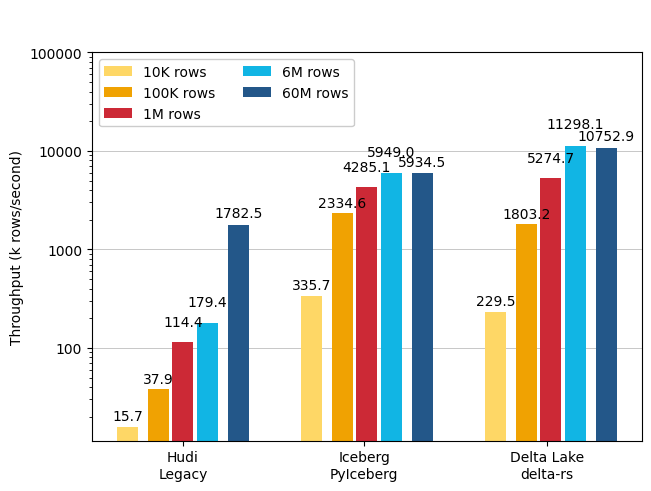
\includegraphics[width=\textwidth]{figures/7-appendix/results_diagrams/read/hudi_iceberg_delta/read_throughput_4_core.png}
        \caption[Histogram of the read experiment - Throughput - 4 CPU cores]{Histogram in log-scale of the read experiment results expressed as throughput. The experiment was performed with four \glstext{CPU} cores.}
        \label{fig:appx_res_read_throughput_4_cores_HID}
    \end{minipage}
\end{figure}

\begin{figure}
    \centering
    \begin{minipage}[b]{\textwidth}
        \centering
        \captionof{table}[Read experiment - Throughput - 8 CPU cores]{Read experiment results expressed as throughput. The experiment was performed with eight \glstext{CPU} cores.}
        \label{tbl:appx_res_read_throughput_8_cores_HID}
        \begin{tabular}{c r S[table-format=5.5] S[table-format=5.5] S[table-format=5.5]} 
            \toprule
            \multirow{2}{*}{{Pipeline\Tstrut\Bstrut}} & \multirow{2}{*}{{\thead{Number\\ of rows}}} & {\multirow{2}{*}{{\thead{Throughput \\ (k rows/second)}}}} & \multicolumn{2}{c}{{\thead{Throughput (k rows/second) \\95\% Confidence Interval}}}\\
                                                      &                                             &                                                          & {low} & {high}\\
            \midrule
            \multirow{5}{4em}{Hudi\\Legacy}         &  10K  &     15.94066  &     15.81039  &     16.06327  \\
                                                    & 100K  &     37.56087  &     37.42290  &     37.68999  \\
                                                    &   1M  &    119.72981  &    116.03188  &    122.82554  \\
                                                    &   6M  &    179.42515  &    177.76438  &    180.88757  \\
                                                    &  60M  &   1810.36775  &   1796.11454  &   1823.66790  \\
            \midrule
            \multirow{5}{4em}{Iceberg\\PyIceberg}   &  10K  &    589.51881  &    552.40208  &    625.87190  \\
                                                    & 100K  &   2343.10833  &   2233.18992  &   2441.60741  \\
                                                    &   1M  &   4308.14374  &   4249.77575  &   4361.60798  \\
                                                    &   6M  &   6782.33584  &   6707.34851  &   6852.17157  \\
                                                    &  60M  &   6787.94365  &   6715.99213  &   6850.14093  \\
            \midrule
            \multirow{5}{4em}{Delta Lake\\delta-rs} &  10K  &    231.78314  &    194.95245  &    257.55578  \\
                                                    & 100K  &   1829.91095  &   1765.22267  &   1887.20060  \\
                                                    &   1M  &   5744.05636  &   5608.98588  &   5888.36778  \\
                                                    &   6M  &  12070.77705  &  11742.93447  &  12355.35882  \\
                                                    &  60M  &  20378.27302  &  19652.71007  &  20981.07517  \\
            \bottomrule
        \end{tabular}
    \end{minipage}
    \begin{minipage}[b]{\textwidth}
        \centering
        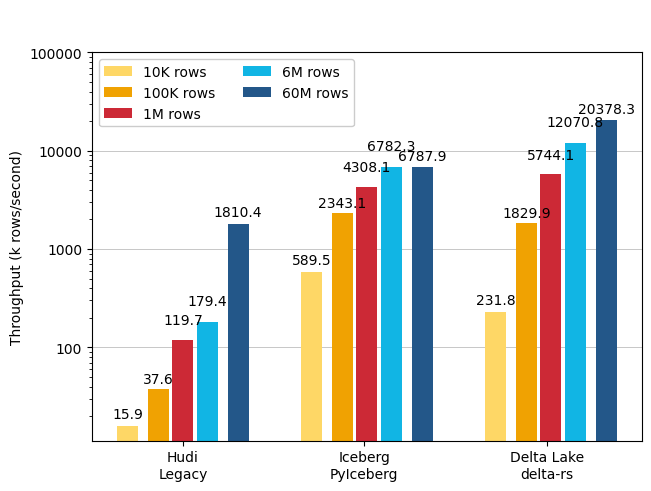
\includegraphics[width=\textwidth]{figures/7-appendix/results_diagrams/read/hudi_iceberg_delta/read_throughput_8_core.png}
        \caption[Histogram of the read experiment - Throughput - 8 CPU cores]{Histogram in log-scale of the read experiment results expressed as throughput. The experiment was performed with eight \glstext{CPU} cores.}
        \label{fig:appx_res_read_throughput_8_cores_HID}
    \end{minipage}
\end{figure}